% \documentclass[
%     table,
%     12pt,
%     oneside,
%     a4paper,
%     italian
% ]{book}

\documentclass{book}

\usepackage[a4paper, margin=3cm]{geometry} % margin
\usepackage{lipsum} % lipsum
\usepackage{courier}
\renewcommand*\familydefault{\ttdefault}
\usepackage[T1]{fontenc}
\usepackage{graphicx} % images
\usepackage{hyperref}

\usepackage[italian]{babel} % italian

\usepackage{everysel}
\EverySelectfont{%
\fontdimen2\font=0.4em% interword space
\fontdimen3\font=0.2em% interword stretch
\fontdimen4\font=0.1em% interword shrink
\fontdimen7\font=0.1em% extra space
\hyphenchar\font=`\-% to allow hyphenation
}

% \pagestyle{headings}
\pagenumbering{center}

\usepackage{fancyhdr}
\pagestyle{fancy}
\fancyhf{} % clear default headers and footers
\fancyhead[L]{\leftmark} % left header: section title
\fancyfoot[C]{\thepage}

\usepackage[toc, acronym, automake]{glossaries}

\usepackage{float} % image position

\usepackage{minted} % code

\newcommand{\myUni}{Università degli Studi di Padova}
\newcommand{\myDepartment}{Dipartimento di Matematica "Tullio Levi-Civita"}
\newcommand{\myFaculty}{Corso di Laurea in Informatica}
\newcommand{\myTitle}{Sviluppo di un Middleware basato su Spring per l'Integrazione di Flussi di Dati}
\newcommand{\myTitleEng}{Development of Spring-Based Middleware for Data Flow Integration}
\newcommand{\myDegree}{Tesi di Laurea Triennale}
\newcommand{\profTitle}{Prof.}
\newcommand{\myProf}{Zanella Marco}
\newcommand{\graduateTitle}{Laureando}
\newcommand{\myName}{Baldo Leonardo}
\newcommand{\myStudentID}{2042372}
\newcommand{\myAA}{2024-2025}
\newcommand{\myLocation}{Padova}
\newcommand{\myTime}{\today}

% \chapter*{Acronimi}

% \paragraph{DB} Database
% \paragraph{DBMS} Database Management System
% \paragraph{IDE} Integrated Development Environment
% \paragraph{JVM} Java Virtual Machine
% \paragraph{SQL} Structured Query Language

% \newpage

\newacronym{DBMS}{DBMS}{Database Management System}
\newacronym{EIP}{EIP}{Enterprise Integration Patterns}
\newacronym{IoT}{IoT}{Internet of Things}
\newacronym{JAR}{JAR}{Java Archive}
\newacronym{JVM}{JVM}{Java Virtual Machine}
\newacronym{POM}{POM}{Project Object Model}
\newacronym{XML}{XML}{eXtensible Markup Language}


% \chapter*{Glossario}

% \paragraph{Open source} In informatica, con l'espressione open source si indica un software distribuito, generalmente in via gratuita, sotto i termini di una licenza open source, che ne concede lo studio, l'utilizzo, la modifica e la redistribuzione. Questo modello si pone in contrapposizione con l'idea di software proprietario che permette le sopracitate concessioni solo secondo i termini dettati dal detentore del copyright.

% \paragraph{JVM} La macchina virtuale Java (detta anche Java Virtual Machine o JVM) è il componente della piattaforma Java responsabile per l'esecuzione dei programmi in formato bytecode. La JVM viene utilizzata per eseguire codice Java.

% \newpage

\newglossaryentry{Middleware}{
    name={Middleware},
    description={Il middleware è un software che funge da strato intermedio tra le applicazioni e le componenti sottostanti, come ad esempio sistemi operativi, database o hardware, facilitando la comunicazione, l'integrazione e la gestione delle risorse nei sistemi distribuiti. Il suo ruolo primario è quello di nascondere la complessità dell'infrastruttura sottostante, garantendo interoperabilità, scalabilità e sicurezza}    
}

\newglossaryentry{Open Source}{
    name={Open Source},
    description={software distribuito, generalmente in via gratuita, sotto i termini di una licenza open source}
}

\newglossaryentry{Topic Kafka}{
    name={Topic Kafka},
    description={I Topic di Kafka sono le categorie utilizzate per organizzare i messaggi. Ogni topic ha un nome unico per l'intero cluster Kafka.
    I messaggi vengono inviati e letti da argomenti specifici. I produttori scrivono dati negli argomenti e i consumatori leggono dati dagli argomenti. 
    In Kafka, gli argomenti sono partizionati e replicati attraverso i broker per tutta l'implementazione.  I broker si riferiscono a ciascuno dei nodi di un cluster Kafka. Le partizioni sono importanti perché permettono la parallelizzazione degli argomenti, consentendo un elevato throughput dei messaggi}
}

\newglossaryentry{Visual Studio Code}{
    name={Visual Studio Code},
    description={editor di codice sorgente sviluppato da Microsoft per Windows, Linux e macOS. È un software libero e gratuito per uso personale e commerciale, anche se la versione ufficiale è sotto una licenza proprietaria. Permette di installare estensioni che aggiungono ulteriori funzionalità}
}

\makeglossaries

\begin{document}
    \let\clearpage\relax
    \let\cleardoublepage\relax

    \frontmatter
    \input{preface/title_page}
    \thispagestyle{empty}

\vspace*{\fill}
{\small\noindent\textcopyright\ \myName, \myTime. Tutti i diritti riservati. \myDegree: "\textit{\myTitle}", \myUni, \myDepartment.}

\newpage

    \chapter*{Ringraziamenti}

Desidero esprimere la mia gratitudine a tutti i professori che mi hanno formato durante il percorso di studio. In particolare desidero ringraziare il professor \myProf, mio relatore, per l'aiuto, la disponibilità e il sostegno che mi ha dato durante la stesura della tesi. \\ \\
Vorrei anche ringraziare, con affetto, la mia famiglia per il loro sostegno e la loro presenza durante gli anni di studio. \\ \\
Infine ringrazio tutti i miei amici, soprattutto i miei compagni di corso Fabio, Nicola e Samuele, per i bellissimi e diventertissimi anni trascorsi insieme e le infinite risate. \\ \\
\noindent{\myLocation, \myTime}
\hfill \textit{\myName}

\newpage

    \chapter*{Abstract}

Il presente documento descrive il lavoro svolto durante il periodo di stage, dalla durata di trecentoventi ore, dal laureando \myName\; presso l'azienda SyncLab S.r.l. \\
Il progetto di stage svolto riguarda lo studio e l'implementazione di \textit{\gls{Middleware}}, in particolar modo il \textit{framework} \nameref{Spring}.
L'applicazione da sviluppare dovrà leggere i dati da un \gls{Topic Kafka}, arricchirli con dati presenti su un \textit{database} e caricare il dato finale su un altro \gls{Topic Kafka}. \\
Prima di iniziare con lo sviluppo effettivo del progetto è stato svolto uno studio approfondito delle tecnologie e degli strumenti coinvolti, i quali verranno analizzati nei successivi capitoli.

\newpage

    \tableofcontents
\newpage

\begingroup

    % Figures list
    \listoffigures
    % \vspace*{8ex}

    % Tables list
    \listoftables
\endgroup

\newpage


    

    \mainmatter
    \chapter{Introduzione}

\section{L'azienda}
L'esperienza di tirocinio svolta dal laureando ha avuto luogo negli uffici della sede veronese dell'azienda SyncLab S.r.l.\footnote{SyncLab S.r.l. - URL: \url{https://synclab.it/home}} \\
Sync Lab è una Innovative Company attenta ai paradigmi della trasformazione digitale che realizza prodotti e soluzioni per diversi mercati quali: Sanità, Industria, Energia, Telco, Finanza e Trasporti \& Logistica. \\
L'offerta di consulenza specialistica, sintesi di circa 20 anni nel settore IT e la forte competenza in diversi domini tecnologici, aiutano il cliente a dominare i nuovi trend e le sfide che ne derivano, quali: GDPR, Big Data, Cloud Computing, \acrshort{IoT}, Mobile e Cyber Security.
In questo scenario Sync Lab si posiziona come uno dei più importanti system integrator nel panorama italiano delle aziende ICT.
\begin{figure}[h]
    \centering
    
\includegraphics[width=0.4\textwidth]{assets/synclab.png}
    \caption{Synclab S.r.l.}
\end{figure}

\section{Organizzazione del testo}
\subsection{Struttura del testo}
Il presente documento è suddiviso in sei capitoli il cui contenuto è brevemente
riassunto in seguito:
\paragraph{Il secondo capitolo} è composto da un'introduzione al progetto, dall'organizzazione del testo e dall'analisi preventiva dei rischi
\paragraph{Il terzo capitolo} è dedicato agli obiettivi e all'analisi dei requisiti
\paragraph{Il quarto capitolo} spiega la parte teorica del progetto
\paragraph{Il quinto capitolo} spiega la parte pratica del progetto
\paragraph{Il sesto capitolo} contiene le conclusioni

\subsection{Convenzioni tipografiche}
In merito alla redazione del presente documento, sono state adottate le seguenti
convenzioni tipografiche:
\begin{itemize}
    \item gli acronimi, le abbreviazioni e i termini ambigui o di uso non comune menzionati vengono definiti nel glossario, situato alla fine del presente documento;
    \item i termini particolarmente rilevanti in una sezione e quelli in lingua straniera non di uso comune o facenti parti del gergo tecnico sono evidenziati con il carattere \textit{corsivo}, fatta eccezione per le occorrenze presenti nei titoli delle sezioni o nelle didascalie;
    \item i comandi di terminale, i frammenti di codice sorgente e i nomi di file o \textit{directory} sono evidenziati con il carattere monospaziato.
\end{itemize}

\newpage

    \chapter{Descrizione dello Stage}

\section{Introduzione al progetto}
Lo scopo principale di questo tirocinio sarà lo studio e l'implementazione di \gls{Middleware}. Principalmente verrà sviluppata con il framework \nameref{sec:Spring} (in particolare SpringBoot, Spring Data/JPA e SprintBatch), inoltre confrontarla con la piattaforma Apache Flink, se possibile.
L'applicazione da sviluppare dovrà leggere i dati da un \gls{Topic Kafka}, arricchirli con dati presenti su \nameref{sec:PostgreSQL} e caricare il dato finale su un altro \gls{Topic Kafka}.
Pertanto, il compito dello studente sarà quello di studiare, progettare, sviluppare e implementare tutte queste funzionalità sulle tecnologie sopra riportate.

\section{Organizzazione del lavoro}
\dots

\section{Analisi preventiva dei rischi}
\dots

\newpage

    \chapter{Analisi dei Requisiti}

\section{Obiettivi dello stage}

\subsection*{Notazione}
Si farà riferimento ai requisiti secondo leseguenti notazioni:
\begin{itemize}
    \item \textbf{O} per i requisiti obbligatori, vincolanti in quanto obiettivo primario richiesto dal committente;
    \item \textbf{D} per i requisiti desiderabili, non cinvolanti o strettamente necessari, ma dal riconoscibile valore aggiunto;
    \item \textbf{F} per i requisiti facoltativi, rappresenanti valore aggiunto non strettamente competitivo.
\end{itemize}
Le sigle precedentemente indicate saranno seguite da una coppia sequenziale di numeri, identificativo del requisito.

\subsection*{Obiettivi fissati}
Si prevede lo svolgimento dei seguenti obiettivi:
\begin{itemize}
    \item Obbligatori
    \begin{itemize}
        \item O01: Implementazione flusso mediante \nameref{sec:Spring};
        \item O02: Relazione tecnica che descriva le scelte tecniche prese durante il percorso e le motivazioni a riguardo;
        \item \dots
    \end{itemize}
    \item Desiderabili
    \begin{itemize}
        \item D01: Implementazione flusso mediante Apache Flink;
        \item D02: Affrontare un'analisi comparativa usando metriche ben precise e coerenti con il contesto applicativo
    \end{itemize}
    \item Facoltativi
    \begin{itemize}
        \item F01: Effettuare dei test di performance mediante strumenti di misurazione dedicati;
        \item F02: Implementare il flusso anche su tecnologie alternative (Apache Camel, Apache NiFi)
    \end{itemize}
\end{itemize}

\section{Tracciamento dei requisiti}

\section{Tabella dei requisiti}

\begin{table}[H]
\centering
\begin{tabular}{|l|l|l|}
\hline
Requisito & Descrizione & Stato \\ \hline
asd & asd & asd \\ \hline
asd & asd &  \\ \hline
asd &  &  \\ \hline
\end{tabular}
\caption{Tabella requisiti}
\label{}
\end{table}

asdasd


\newpage

    \chapter{Microservizi}

Nell'ingegneria del software, l'architettura a microservizi è un modello architettonico che organizza un'applicazione in un insieme di servizi a grana fine e liberamente accoppiati che comunicano attraverso protocolli leggeri. Questo modello è caratterizzato dalla capacità di sviluppare e distribuire servizi in modo indipendente, migliorando la modularità, la scalabilità e l'adattabilità. Tuttavia, introduce un'ulteriore complessità, in particolare nella gestione dei sistemi distribuiti e della comunicazione tra servizi, rendendo l'implementazione iniziale più impegnativa rispetto a un'architettura monolitica. \\ \\
Non esiste una definizione unica e universalmente condivisa di microservizi. Tuttavia, essi sono generalmente caratterizzati da un'attenzione particolare alla modularità, con ogni servizio progettato intorno a una specifica funzionalità aziendale. Questi servizi sono liberamente accoppiati, distribuibili in modo indipendente e spesso sviluppati e scalati separatamente, consentendo una maggiore flessibilità e agilità nella gestione di sistemi complessi. L'architettura a microservizi è strettamente associata a principi quali la progettazione guidata dal dominio, la decentralizzazione dei dati e della governance e la flessibilità di utilizzare tecnologie diverse per i singoli servizi, in modo da soddisfare al meglio i loro requisiti. 

\newpage

    \chapter{Codifica}

\section{Tecnologie e strumenti}

\subsection{Linguaggio e piattaforma}
Il \textit{middleware} è stato sviluppato in \nameref{Java} e gestito tramite \nameref{Apache Maven} come \textit{build tool}, che si occupa della risoluzione delle dipendenze, della compilazione e del \textit{packaging} dell'applicazione in un \textcolor{purple}{jar} eseguibile.

\subsubsection{Java}
\label{Java}
Java è un linguaggio di programmazione ad alto livello, orientato agli oggetti e a tipizzazione statica, che si appoggia sull'omonima piattaforma \textit{software} di esecuzione, specificamente progettato per essere il più possibile indipendente dalla piattaforma \textit{hardware} di esecuzione (tramite compilazione in \textit{bytecode} prima e interpretazione poi da parte di una \acrshort{JVM}).
\begin{figure}[H]
    \centering
    
\includegraphics[width=0.2\textwidth]{assets/java.png}
    \caption{Java}
\end{figure}

\subsubsection{Apache Maven}
\label{Apache Maven}
Apache Maven è uno strumento di gestione di progetti \textit{software} basati su \nameref{Java} e \textit{build automation}. \\
Maven usa un costrutto conosciuto come \acrshort{POM}; un file \acrshort{XML} che descrive le dipendenze fra il progetto, le varie versioni di librerie necessarie e le dipendenze fra di esse. In questo modo si separano le librerie dalla \textit{directory} di progetto utilizzando questo file descrittivo per definirne le relazioni. \\
Maven effettua automaticamente il \textit{download} di librerie \nameref{Java} e \textit{plug-in} Maven dai vari \textit{repository} definiti scaricandoli in locale o in un \textit{repository} centralizzato lato sviluppo. Questo permette di recuperare in modo uniforme i vari file \acrshort{JAR} e di poter spostare il progetto indipendentemente da un ambiente all'altro avendo la sicurezza di utilizzare sempre le stesse versioni delle librerie.
\begin{figure}[H]
    \centering
    
\includegraphics[width=0.4\textwidth]{assets/apacheMaven.png}
    \caption{Apache Maven}
\end{figure}

\subsection{Framework applicativo}
Il progetto si basa principalmente sul framework Spring, in particolare i seguenti moduli:
\begin{itemize}
    \item \textbf{Spring Boot:} per semplificare la configurazione e l'avvio di applicazioni Java
    \item \textbf{Spring Data JPA:} per la persistenzadei dati
    \item \textbf{Spring Kafka:} per l'integrazione dichiarativa con \nameref{Apache Kafka} (consumer, producer, listener)
\end{itemize}

\subsubsection{Spring}
\label{Spring}
Spring è un framework \gls{Open Source} per lo sviluppo di applicazioni su piattaforma Java.
A questo framework sono associati tanti altri progetti, che hanno nomi composti come Spring Boot, Spring Data JPA e Spring Kafka. 
Questi progetti sono stati ideati per fornire funzionalità aggiuntive al framework.
\begin{figure}[H]
    \centering
    
\includegraphics[width=0.4\textwidth]{assets/spring.png}
    \caption{Spring}
\end{figure}

\subsection{Infrastruttura di supporto}
L'ambiente di sviluppo è orchestrato tramite Docker e Docker Compose, secondo la definizione riportata nel file \textcolor{purple}{docker-compose.yml}, che avvia tre servizi containerizzati:
\begin{itemize}
    \item \textbf{PostgreSQL:} il \textit{database} relazionale che ospita i dati di arricchimento;
    \item \textbf{Apache Kafka:} configurato in modalità KRaft (Kafka Raft), l'architettura più recente che elimina la dipendenza da Apache ZooKeeper per il coordinamento del \textit{cluster}, unificando i ruoli di \textit{broker} e \textit{controller} in un singolo nodo (scelta adeguata a un ambiente di sviluppo locale a singolo nodo);
    \item \textbf{Kafka UI:} un'interfaccia web (esposta sulla porta \textcolor{purple}{8081}) che consente di ispezionare topic, partizioni, messaggi e \textit{consumer group} senza dover ricorrere alla sola riga di comando.
\end{itemize}
Questa infrastruttura consente di riprodurre in locale, in modo rapido e ripetibile, un ambiente rappresentativo di un \textit{deployment} di produzione, mantenendo però la semplicità necessaria in fase di sviluppo e test.

\subsubsection{Docker}
\label{Docker}
Docker è un popolare \textit{software} libero che utilizza la virtualizzazione a livello di sistema operativo per eseguire applicazioni in ambienti isolati chiamati \textit{container}. \\
I container Docker sono un'estensione dei \textit{container} del sistema operativo. Docker supporta sia i container Linux che quelli Windows. È possibile utilizzare Docker con container Linux anche nei sistemi Windows e MacOS grazie a tecniche di virtualizzazione.
\begin{figure}[H]
    \centering
    
\includegraphics[width=0.4\textwidth]{assets/docker.png}
    \caption{Docker}
\end{figure}

\subsubsection{PostgreSQL}
\label{PostgreSQL}
PostgreSQL è un completo \acrshort{DBMS} ad oggetti pubblicato con licenza libera (stile Licenza BSD). Spesso abbreviato come "Postgres", sebbene questo sia un nome vecchio dello stesso progetto, è una reale alternativa sia rispetto ad altri prodotti liberi come MySQL, Firebird SQL e MaxDB che a quelli a codice chiuso come Oracle, IBM Informix o DB2 ed offre caratteristiche uniche nel suo genere che lo pongono per alcuni aspetti all'avanguardia nel settore delle basi di dati. 
\begin{figure}[H]
    \centering
    
\includegraphics[width=0.3\textwidth]{assets/postgresql.png}
    \caption{PostgreSQL}
\end{figure}

\subsubsection{Apache Kafka}
\label{Apache Kafka}
Apache Kafka è una piattaforma \gls{Open Source} di \textit{stream processing} scritta in Java e Scala e sviluppata dall'Apache Software Foundation. Il progetto mira a creare una piattaforma a bassa latenza ed alta velocità per la gestione di \textit{feed} dati in tempo reale. \\
Questo progetto viene usato principalmente per tutte le applicazioni di elaborazioni di \textit{stream} di dati in tempo reale.
\begin{figure}[H]
    \centering
    
\includegraphics[width=0.4\textwidth]{assets/apacheKafka.png}
    \caption{Apache Kafka}
\end{figure}

\section{Progettazione}
\label{Progettazione}
Prima di procedere all'implementazione, sono state definite alcune scelte progettuali riguardanti il modello dei dati, la struttura dei \gls{Topic Kafka} e la gestione degli errori.

\subsection{Modello dei dati}
Sono stati definiti tre tipi di oggetti, ciascuno con una responsabilità precisa:
\begin{itemize}
    \item \textcolor{purple}{OrderEvent}: rappresenta il messaggio grezzo in ingresso, contenente un identificativo dell'ordine (\textcolor{purple}{orderId}), un riferimento al cliente (\textcolor{purple}{customerId}) e i dati dell'ordine stesso (\textcolor{purple}{product}, \textcolor{purple}{amount});
    \item \textcolor{purple}{Customer}: entità contenente i dati del cliente (\textcolor{purple}{fullName}, \textcolor{purple}{email}, \textcolor{purple}{city}) necessari all'arricchimento;
    \item \textcolor{purple}{EnrichedOrder}: rappresenta il messaggio finale pubblicato in uscita, che unisce i dati dell'ordine originario con i dati del cliente recuperati da \nameref{PostgreSQL}, più un \textit{timestamp} (\textcolor{purple}{enrichedAt}) che documenta il momento dell'arricchimento.
\end{itemize}
Questa separazione segue il pattern \nameref{Content Enricher}: il messaggio in ingresso è  "povero", mentre il contratto in uscita è "arricchito" con informazioni che il produttore originario dell'evento non possiede.

\subsection{Progettazione dei topic Kafka}
Sono stati previsti tre topic, ciascuno con un numero di partizioni proporzionato al ruolo previsto:
\begin{table}[H]
    \setlength{\tabcolsep}{10pt} % Default value: 6pt
    \def\arraystretch{1.5} % Default value: 1
    \centering
    \begin{tabular}{|l|l|p{0.45\linewidth}|}
        \hline
        \textbf{Topic} & \textbf{Partizioni} & \textbf{Ruolo} \\ \hline
        \textcolor{purple}{orders-input} & 3 & ingresso degli ordini grezzi \\ \hline
        \textcolor{purple}{orders-output} & 3 & uscita degli ordini arricchiti \\ \hline
        \textcolor{purple}{orders-input-dlq} & 1 & dead letter queue per ordini non arricchibili \\ \hline
    \end{tabular}
    \caption{Tabella dei topic}
    \label{Tabella dei topic}
\end{table}
\noindent
Il numero di partizioni maggiore per i topic di flusso principale (\textcolor{purple}{orders-input}, \textcolor{purple}{orders-output}) consente il parallelismo in lettura/scrittura descritto in \ref{Event Streaming}.
La singola partizione per la \acrshort{DLQ} riflette invece un volume atteso più basso e la priorità data alla semplicità di ispezione rispetto al parallelismo.

\subsection{Progettazione del flusso di elaborazione}
Il flusso di elaborazione è stato progettato secondo la seguente sequenza logica:
\begin{enumerate}
    \item un evento ordine viene pubblicato su \textcolor{purple}{orders-input};
    \item il middleware consuma il messaggio;
    \item il middleware tenta di recuperare i dati del cliente corrispondente su \nameref{PostgreSQL};
    \begin{enumerate}
        \item se il cliente viene trovato, viene composto il messaggio arricchito e pubblicato su \textcolor{purple}{orders-output};
        \item se il cliente non viene trovato, l'evento originario viene instradato su \textcolor{purple}{orders-input-dlq}, secondo il pattern \nameref{Dead Letter Channel} descritto in \ref{Dead Letter Channel};
    \end{enumerate}
\end{enumerate}
\begin{figure}[H]
    \centering
    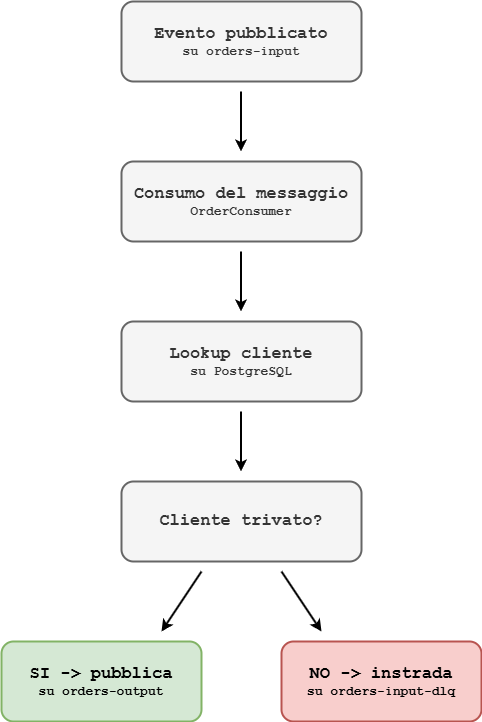
\includegraphics[width=0.5\textwidth]{assets/flusso.drawio.png}
    \caption{Flusso di elaborazione}
\end{figure}
Questa progettazione garantisce che, in caso di arresto anomalo dell'applicazione tra la lettura del messaggio e la sua elaborazione completa, il messaggio venga riletto al riavvio (semantica at-least-once, discussa in \ref{Semantica di consegna}), evitando così perdite di dati a scapito di un'eventuale elaborazione duplicata.

\newpage

    \chapter{Conclusioni}
\label{Conclusioni}

% \section{Sintesi del lavoro svolto}
% Il presente lavoro ha affrontato lo studio, la progettazione e l'implementazione di un \textit{middleware} basato sul pattern \nameref{Content Enricher}, realizzato tramite \nameref{Spring} (Spring Boot, Spring Data JPA, Spring Kafka) secondo quanto descritto nei capitoli~\ref{Middleware} e~\ref{Codifica}. Il sistema legge eventi da un \textit{topic} \nameref{Apache Kafka} sorgente, li arricchisce con dati letti da \nameref{PostgreSQL} e pubblica il risultato su un \textit{topic} di destinazione, gestendo esplicitamente i casi di dato mancante tramite il pattern \nameref{Dead Letter Channel}. Gli obiettivi obbligatori O01-O03 definiti in \ref{Obiettivi fissati} risultano pertanto soddisfatti, come riportato nelle tabelle di tracciamento dei requisiti.

% \section{Limiti e sviluppi futuri}
% Due obiettivi definiti in fase di analisi dei requisiti non sono stati portati a esecuzione, per priorità assegnata allo sviluppo dell'implementazione principale nel tempo a disposizione del tirocinio: l'implementazione equivalente in \textbf{Apache Flink} (D02, RFD-07, \ref{Ambito del confronto con Apache Flink}) e l'esecuzione dei \textbf{test di performance} (F01, RFF-08, \ref{Ambito dei test di performance}). \\ \\
% Per entrambi, il presente lavoro definisce comunque una base pronta all'esecuzione: il Capitolo~\ref{Middleware Chapter} presenta i concetti teorici di Flink e un confronto concettuale con l'approccio Spring adottato (\ref{Confronto Spring Flink}), mentre il Capitolo~\ref{Codifica Chapter} ne definisce la progettazione concreta (\ref{Progettazione teorica Flink}) e gli strumenti con cui si eseguono i test di performance (\ref{Strumenti per i test di performance}). Una naturale prosecuzione del lavoro realizza questa pipeline e applica ad entrambe le implementazioni la medesima metodologia di valutazione definita nel Capitolo~\ref{Middleware Chapter}, permettendo un confronto fondato su dati anziché su sole considerazioni architetturali.

\newpage


    \backmatter
    \printglossary[type=\acronymtype, title=Acronimi]
    \printglossary[type=main, title=Glossario]
    \glsaddallunused
    \newpage
    % % \chapter*{Acronimi}

% \paragraph{DB} Database
% \paragraph{DBMS} Database Management System
% \paragraph{IDE} Integrated Development Environment
% \paragraph{JVM} Java Virtual Machine
% \paragraph{SQL} Structured Query Language

% \newpage

\newacronym{DBMS}{DBMS}{Database Management System}
\newacronym{EIP}{EIP}{Enterprise Integration Patterns}
\newacronym{IoT}{IoT}{Internet of Things}
\newacronym{JAR}{JAR}{Java Archive}
\newacronym{JVM}{JVM}{Java Virtual Machine}
\newacronym{POM}{POM}{Project Object Model}
\newacronym{XML}{XML}{eXtensible Markup Language}


    % % \chapter*{Glossario}

% \paragraph{Open source} In informatica, con l'espressione open source si indica un software distribuito, generalmente in via gratuita, sotto i termini di una licenza open source, che ne concede lo studio, l'utilizzo, la modifica e la redistribuzione. Questo modello si pone in contrapposizione con l'idea di software proprietario che permette le sopracitate concessioni solo secondo i termini dettati dal detentore del copyright.

% \paragraph{JVM} La macchina virtuale Java (detta anche Java Virtual Machine o JVM) è il componente della piattaforma Java responsabile per l'esecuzione dei programmi in formato bytecode. La JVM viene utilizzata per eseguire codice Java.

% \newpage

\newglossaryentry{Middleware}{
    name={Middleware},
    description={Il middleware è un software che funge da strato intermedio tra le applicazioni e le componenti sottostanti, come ad esempio sistemi operativi, database o hardware, facilitando la comunicazione, l'integrazione e la gestione delle risorse nei sistemi distribuiti. Il suo ruolo primario è quello di nascondere la complessità dell'infrastruttura sottostante, garantendo interoperabilità, scalabilità e sicurezza}    
}

\newglossaryentry{Open Source}{
    name={Open Source},
    description={software distribuito, generalmente in via gratuita, sotto i termini di una licenza open source}
}

\newglossaryentry{Topic Kafka}{
    name={Topic Kafka},
    description={I Topic di Kafka sono le categorie utilizzate per organizzare i messaggi. Ogni topic ha un nome unico per l'intero cluster Kafka.
    I messaggi vengono inviati e letti da argomenti specifici. I produttori scrivono dati negli argomenti e i consumatori leggono dati dagli argomenti. 
    In Kafka, gli argomenti sono partizionati e replicati attraverso i broker per tutta l'implementazione.  I broker si riferiscono a ciascuno dei nodi di un cluster Kafka. Le partizioni sono importanti perché permettono la parallelizzazione degli argomenti, consentendo un elevato throughput dei messaggi}
}

\newglossaryentry{Visual Studio Code}{
    name={Visual Studio Code},
    description={editor di codice sorgente sviluppato da Microsoft per Windows, Linux e macOS. È un software libero e gratuito per uso personale e commerciale, anche se la versione ufficiale è sotto una licenza proprietaria. Permette di installare estensioni che aggiungono ulteriori funzionalità}
}

    \chapter*{Bibliografia}

\section*{Testi}
\dots

\section*{Articoli}
\dots

\section*{Siti web}
Apache Kafka - URL: \url{https://kafka.apache.org/} - \ref{Apache Kafka come servizio di messaggistica} \\ \\
Content Enricher - URL: \url{https://www.enterpriseintegrationpatterns.com/patterns/messaging/DataEnricher.html} - \ref{Content Enricher} \\ \\
Dead Letter Channel - URL: \url{https://www.enterpriseintegrationpatterns.com/patterns/messaging/DeadLetterChannel.html} - \ref{Dead Letter Channel} \\ \\
Enterprise Integration Patterns - URL: \url{https://www.enterpriseintegrationpatterns.com/} - \ref{Enterprise Integration Patterns} \\ \\
Message Channel - URL: \url{https://www.enterpriseintegrationpatterns.com/patterns/messaging/MessageChannel.html} - \ref{Message Channel} \\ \\
Message Translator - URL: \url{https://www.enterpriseintegrationpatterns.com/patterns/messaging/MessageTranslator.html} - \ref{Message Translator} \\ \\
Middleware - URL: \url{https://en.wikipedia.org/wiki/Middleware} - \ref{Middleware} \\ \\
Middleware - URL: \url{https://en.wikipedia.org/wiki/Middleware_(distributed_applications)} - \ref{Middleware} \\ \\
Point-to-Point Channel - URL: \url{https://www.enterpriseintegrationpatterns.com/patterns/messaging/PointToPointChannel.html} - \ref{Point-to-Point Channel} \\ \\

\newpage

    % \printglossaries
    
\end{document}
